\chapter{Ethereum and Blockchain Basics}\label{ch:basics}

In 2009 Satoshi Nakamoto published the Bitcoin whitepaper~\cite{bitcoin} where he described `a purely peer-to-peer version of electronic cash' which `would allow online payments to be sent directly from one party to another without going through a financial institution'. 

Bitcoin was primarily used for fast and low-cost financial transactions which were routed without any bank interference. It was soon realized that its underlying technology, blockchain, could be used for more than transferring financial value. A blockchain is a database that can be shared between a group of non-trusting individuals, without needing a central party to maintain the state of the database. The data in a blockchain is transparent and secured via cryptography. As more advanced blockchain platforms were built on top of Bitcoin~\cite{colored}, in the end of 2014 a blockchain platform which was capable of executing smart contracts was released, called Ethereum~\cite{vitalik}. A smart contract, first referred to as a term by Szabo in \cite{szabo}, is software that is executed on a blockchain and can be used as a framework for secure and trustless computation. 

\section{General Background}
Before getting into the specifics of blockchains and Ethereum, the next section will be used to explain fundamental terms on cryptography (hash functions and public key cryptography) and blockchain.

A blockchain can be described as a list of \textit{blocks} that grows over time. Each block contains various metadata (called \textit{block headers}) and a list of transactions. A block is linked to another block by referencing its \textit{hash}. A blockchain gets formed when each existing block has a valid reference to the previous block. It is the case that as more blocks get added to a blockchain, older blocks and their contents are considered to be more secure.

Any future reference to blockchain terminology such as the contents of a block or a transaction will be specific to the implementations of the Ethereum Platform. The Ethereum Yellowpaper provides details on the formal definitions and contents of each term~\cite{ethereum}.

\subsection{Cryptographic Hash Functions}
A hash function is any function that maps data of arbitrary size to a fixed size string. The result of a hash function is often called the \textit{hash} of its input. Hash functions used in cryptography must fullfil additional security properties and are called \textit{cryptographic hash functions}.

More specifically, a secure cryptographic hash function should satisfy the following properties \cite{Rogaway04cryptographichash-function} (\(H(x)\) refers to the hash of $x$):
\begin{enumerate}
   \item \textbf{Collision Resistance}: It should be computationally infeasible to find $x$ and $y$ such that \(H(x) = H(y)\). 
   \item \textbf{Pre-Image Resistance}: Given \(H(x)\) it should be computationally infeasible to find \(x\).
   \item \textbf{Second Pre-Image Resistance}: Given \(H(x)\) it should be computationally infeasible to find \(x'\) so that \(H(x') = H(x)\). A second preimage attack on a hash function is significantly more difficult than a preimage attack due to the attacker being able to manipulate only one input of the problem. 
\end{enumerate}

Bitcoin uses the SHA-256 cryptographic hash function, while Ethereum uses KECCAK-256 \cite{btchash, ethash}. Ethereum's KECCAK-256 is oftentimes mistakenly referred to as SHA-3 which is inaccurate since SHA3-256 has different padding and thus different values\cite{sha3}.

\subsection{Public Key Cryptography}
Also referred to as Asymmetric Cryptography, it is a system that uses a pair of keys to encrypt and decrypt data. The two keys are called \textit{public} and \textit{private}\footnote{The public key is a number which is derived by elliptic curve multiplication on the private key. The private key is usually a large number known only to its owner. The public key is in the public domain.}. The main advantage of Public Key Cryptography is that it establishes secure communication without the need for a secure channel for the initial exchange of keys between any communicating parties.

The security Public Key Cryptography is based on cryptographic algorithms which are not solvable efficiently due to certain mathematical problems, such as the factorization of large integer numbers for RSA\cite{Rivest:1978:MOD:359340.359342} or calculating the discrete logarithm\footnote{The discrete logarithm $log_{b}a$ is an integer $k$ such that $b^k = a$} for the Elliptic Curve Digital Signature Algorithm (ECDSA), being hard.

Public key cryptography allows for secure communications by achieving:

\begin{enumerate}
    \item \textbf{Confidentiality - A message must not be readable by a third party:} By encrypting the plaintext with recipient's public key, the only way to decrypt it is by using the recipient's private key, which is only known to the recipient, thus achieving confidentiality of the message's transmission. This has the disadvantage that it does not achieve authentication and thus anyone can impersonate the sender.
    \item \textbf{Authentication - The receiver must be able to verify the sender's identity:} By encrypting the plaintext with sender's private key, the only valid decryption can be done with the sender's public key. This authenticates the identity of the sender of the message. This has the disadvantage that the message can be read by any middle-man as the sender's public key is known.
    \item \textbf{Confidentiality and Authenticaton - The receiver must be able to verify the sender's identity and verify that the message was not read by a third party:} The original message gets encrypted with the sender's private key and encrypted again with the recipient's public key. That way, a recipient decrypts the message firstly with their private key, achieving confidentiality, and then verifies the identity of the sender by decrypting with the sender's public key.
    \item \textbf{Integrity - The receiver must be able to verify that the message was not modified during transmission:} Digital signatures is a scheme which allows the recipient to both verify that the message was created by a sender and that the message has not been tampered with. 
    The process is as follows:
    \begin{enumerate}
        \item The sender calculates the hash of the message that they are transmitting and concatenates the message with the hash
        \item The sender encrypts the combined message with their private key and transmits the ciphertext to the receiver  
        \item The receiver decrypts the content of the message with the sender's public key, achieving authentication
        \item The receiver hashes the plaintext and compares the result to the transmitted hash
        \item If the result matches the transmitted hash  then, given that the hashing function used is secure,
        the message has not been tampered with
    \end{enumerate}
    If the sender wanted to also make sure of the confidentiality of the information, they would also encrypt with the receiver's public key after step 2, and similarly the receiver would decrypt with their private key after step 3. This process is often referred to as a sender broadcasting a \textit{signed} message.

\end{enumerate}

\subsection{Some basic features of blockchains} \label{advantages}
A blockchain acts as a distributed immutable public ledger. It can be used to efficiently transfer value between multiple parties without using a trusted intermediary (e.g. a bank in the case of a financial transaction) to settle the transaction. 

% Supplier - Client model in a transaction
Due to the public nature of the ledger, it provides transparency as every transaction can be inspected to verify its associated information. This can be utilized by interested suppliers (e.g. companies) to cultivate trust with their clients or partners by providing them access to the needed functionalities without compromising otherwise private information. There are privacy implications with this however, since companies might not want to disclose all pieces of information to the public. Privacy enabled blockchains which use advanced cryptography to hide transaction information from non-transacting parties already exist \cite{monero, zcash, pivx} . Bitcoin utilizes \textit{pseudonyms} to hide the identity of an individual behind a random address\footnote{An individual can generate multiple addresses from the same private key.}, however research has shown that this is not always a reliable privacy preservation measure~\cite{journals/corr/abs-1107-4524, DBLP:journals/corr/abs-1708-04748}.

Due to the distributed nature of the ledger, it is currently impossible for a party to censor a transaction. This has very powerful implications (e.g. in the case of an authoritarian regime, there is no way for a transaction to be cancelled due to a court order). On the other hand, in the case of theft of private keys, there is no way to prevent an attacker from stealing a victim's funds.  At current scale, transactions on a blockchain have very low costs to execute and very high confirmation speeds \cite{ethpricestats}.

The ledger is secured by the used protocol rules which utilize so called \textit{consensus algorithms}\cite{consensus_algo} to provide transaction finality and immutability. As a result, blockchains can be used to timestamp events in history \cite{ots} which can be utilized to prevent fraud. This feature is incompatible with the flexibility of centralized databases which allow for any past event to be rewritten, which allows for scenarios such as reverting the bank balance of a customer in the case of a mistaken transaction. 

\subsection{Blockchain Types}
In order to tackle the disadvantages mentioned in \ref{advantages}, blockchains that make tradeoffs in decentralization for more 
Blockchains are inspectable and public. Any entity can setup a node, download the full blockchain history and view all the transactions caused by anyone participating in that network. This is one of the main benefits of using a blockchain, transparency.

There are two blockchain categories:
\begin{enumerate}
    \item Public or Permissionless: Low barrier to entry, transparent and immutable.
    \item Private or Permissioned: Federated participation, can obscure certain pieces of data, ability to modify and revert past transactions if needed.
\end{enumerate}

Vitalik Buterin goes indepth in the advantages and disadvantages between private and public blockchains in~\cite{publicprivate}. Due to the scalability and privacy restrictions of public blockchains, corporations can use permissioned blockchain frameworks~\cite{quorum, hyperledger, r3} to include blockchain technology in their processes.

\section{Ethereum Blockchain}
The Ethereum blockchain acts as a transactional state machine. The first state is the \textit{genesis} state referred to as the \textit{genesis block}. After the execution of each transaction, the state changes. Transactions are collated together in \textit{blocks}. 

\begin{figure}[H]
    \centering
    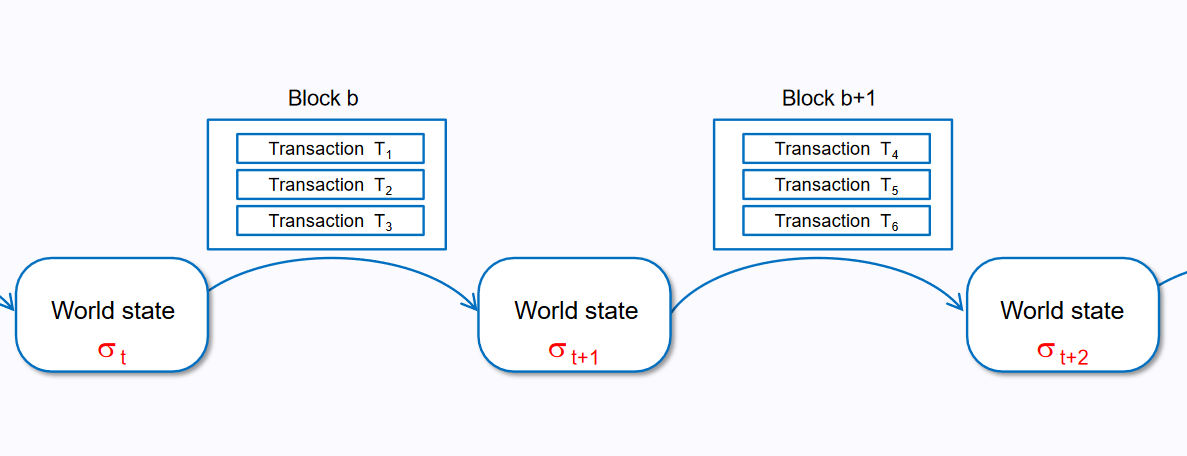
\includegraphics[width=1.0\textwidth]{blockchain_transitions}
    \caption{Ethereum can be seen as a chain of states, from~\cite{visual}}
    \label{fig:worldstate_update}
\end{figure}

A valid state transition requires the appending of a new block to the existing list of blocks. Each block contains transactions and a reference~to the previous block, forming a chain. In Ethereum, the only way for a block to be validated and appended to the list is through a validation process called mining. Mining involves a group of computers, known as miners, expending their computational resources to find the solution to a puzzle. The first miner to find a solution to the puzzle is rewarded with Ether\footnote{The Ethereum network's native currency} and is able to validate their block proposal. This is a process known as \textit{Proof of Work} (PoW) \cite{pow}. 

Due to a large number of miners competing to solve the PoW puzzle, sometimes a miner might solve the PoW at the same time with another miner, but for different block contents. This results in a \textit{fork} of the blockchain. Nodes will accept the first valid block that they receive\footnote{This depends on block propagation time based on bandwith, block-size, connectivity etc.}. Each blockchain protocol has a way to resolve forks and determine which chain is the valid chain. In Ethereum the longest chain is based on total difficulty\footnote{Difficulty is a measure of how much computational effort needs to be given coon average by a mir to solve a PoW puzzle. Total Difficulty is the sum of the difficulties of all blocks until the examined block} which can be found in the \textit{blockheader}. Ethereum is advertised to be using a modification of the GHOST Protocol\cite{GHOST} as its chain selection mechanism which uses \textit{uncle blocks}\footnote{In Bitcoin a block with a valid PoW that arrived to a node after another valid block at the same height is called an orphan because it gets discarded by Bitcoin's algorithm. In Ethereum these blocks do not get discarded; instead they are added to the chain as \textit{uncle blocks} and receive a reduced block reward}. This is contradictory since Ethereum's uncle blocks do not count towards difficulty and as a result, Ethereum does not actually use an adaptation of the GHOST protocol \cite{Gervais:2016:SPP:2976749.2978341}; the uncle reward is just used to reduce miner centralization.

\begin{figure}[H]
    \centering
    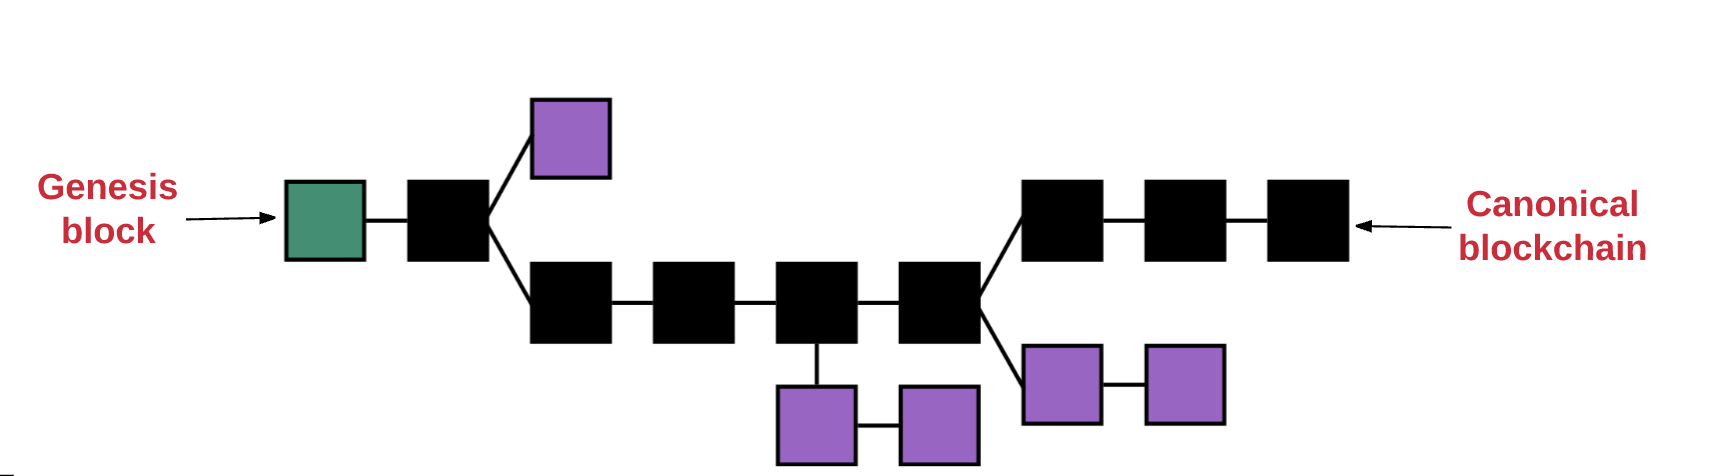
\includegraphics[width=1.0\textwidth]{fork}
    \caption{Blockchain forks: Ethereum's protocol chooses the canonical chain, from \cite{preethi}}
    \label{fig:forking}
\end{figure}

\section{Inside the Ethereum Virtual Machine}
% https://hudsonjameson.com/2017-06-27-accounts-transactions-gas-ethereum/
The \textit{Ethereum Virtual Machine} (EVM) is the runtime environment for Ethereum. It is a Turing Complete State machine, allowing arbitrarily complex computations to be executed on it. Ethereum nodes validate blocks and also run the EVM, which means executing the code that is triggered by the transactions. In this section we go over the internals of the EVM\@. 

\subsection{Accounts}

\subsubsection{World State}
Ethereum's world state is a mapping between addresses of accounts and their states. Full nodes download the blockchain, execute and verify the full result of every transaction since the genesis block. Users should run a full node if they need to execute every transaction in the blockchain or if they need to swiftly query historical data. 

\begin{figure}[H]
    \centering
    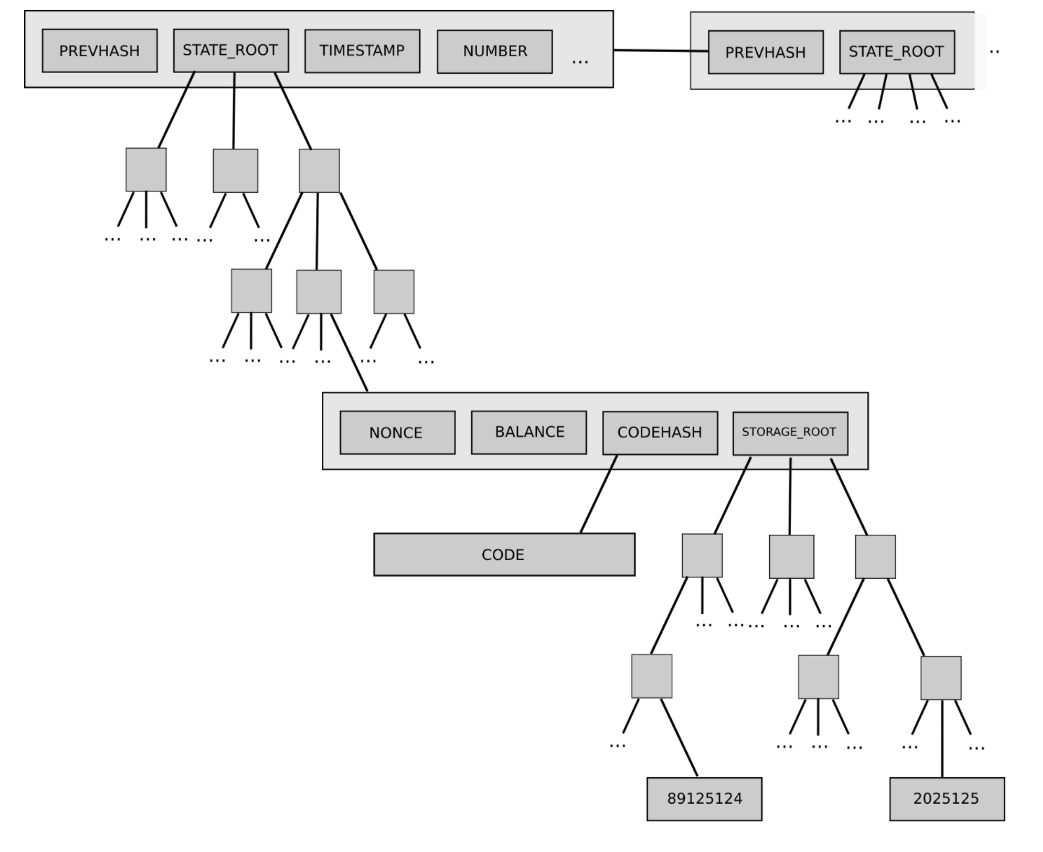
\includegraphics[width=1.0\textwidth]{world_state}
    \caption{The world state of Ethereum, from~\cite{vitalik}}
    \label{fig:worldstate}
\end{figure}

A different kind of node called \textit{light node} exists for cases where there is no need to store all the information. Instead, light nodes use efficient data structures called \textit{Merkle Trees} which allow them to verify the validity of the data of a tree without storing the entire tree. A \textit{Merkle Tree} is a binary tree where each parent node is the hash of its two child nodes\footnote{Exception: Each leaf node represents the hash of a transaction in a block}. 

\begin{figure}[H]
    \centering
    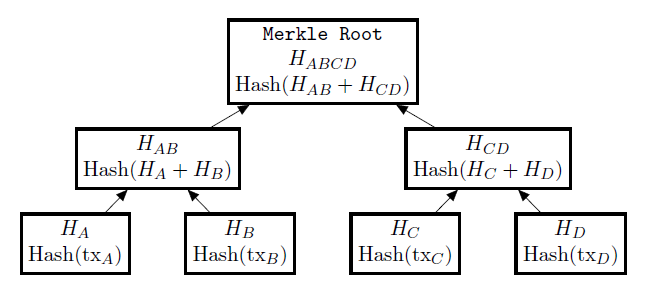
\includegraphics[width=1.0\textwidth]{merkle_tree}
    \caption{Node calculation in a Merkle Tree, from~\cite{smartproperty}}
    \label{fig:merkletree}
\end{figure}

That way, instead of storing the whole tree of transactions, nodes can verify if a transaction was included in a block or not just by checking if the `merkle path' to the merkle root is valid. This is efficient as there are only $O(lg_{2}(n))$ comparisons needed to check the validity of a transaction, as shown in Figure \ref{fig:merkleproof}

\begin{figure}[H]
    \centering
    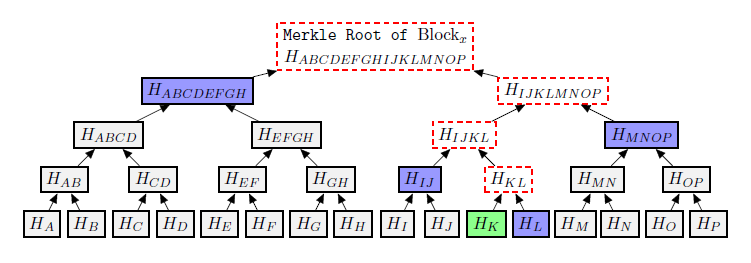
\includegraphics[width=1.0\textwidth]{merkle_proof}:
    \caption{To prove that $H_{k}$ was included in the merkle root of $Block_{x}$ only the blue elements are needed, from \cite{smartproperty}}
    \label{fig:merkleproof}
\end{figure}

\subsubsection{Account State}
An ethereum account is a mapping between an address and an account state. There are two kinds of accounts, \textit{Externally Owned Accounts} (EOA) and \textit{Contract Accounts} (CA).

\begin{figure}[H]
    \centering
    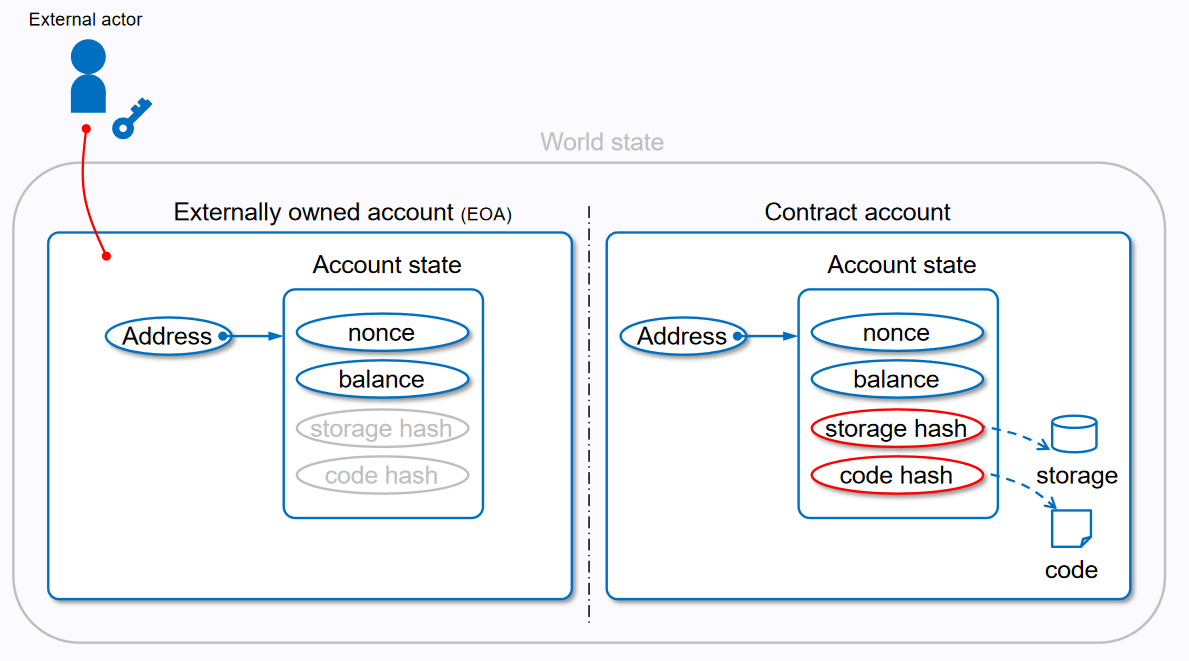
\includegraphics[width=1.0\textwidth]{accounts}
    \caption{EOA is controlled by a Private Key and cannot contain EVM code. CAs contain EVM code and are controlled by the EVM code, from \cite{visual}}
    \label{fig:accounts}
\end{figure}

An EOA is able to send a message to another EOA by signing a transaction with their private key. CAs can make transactions in response to transactions they receive from EOAs. 

\begin{figure}[H]
    \centering
    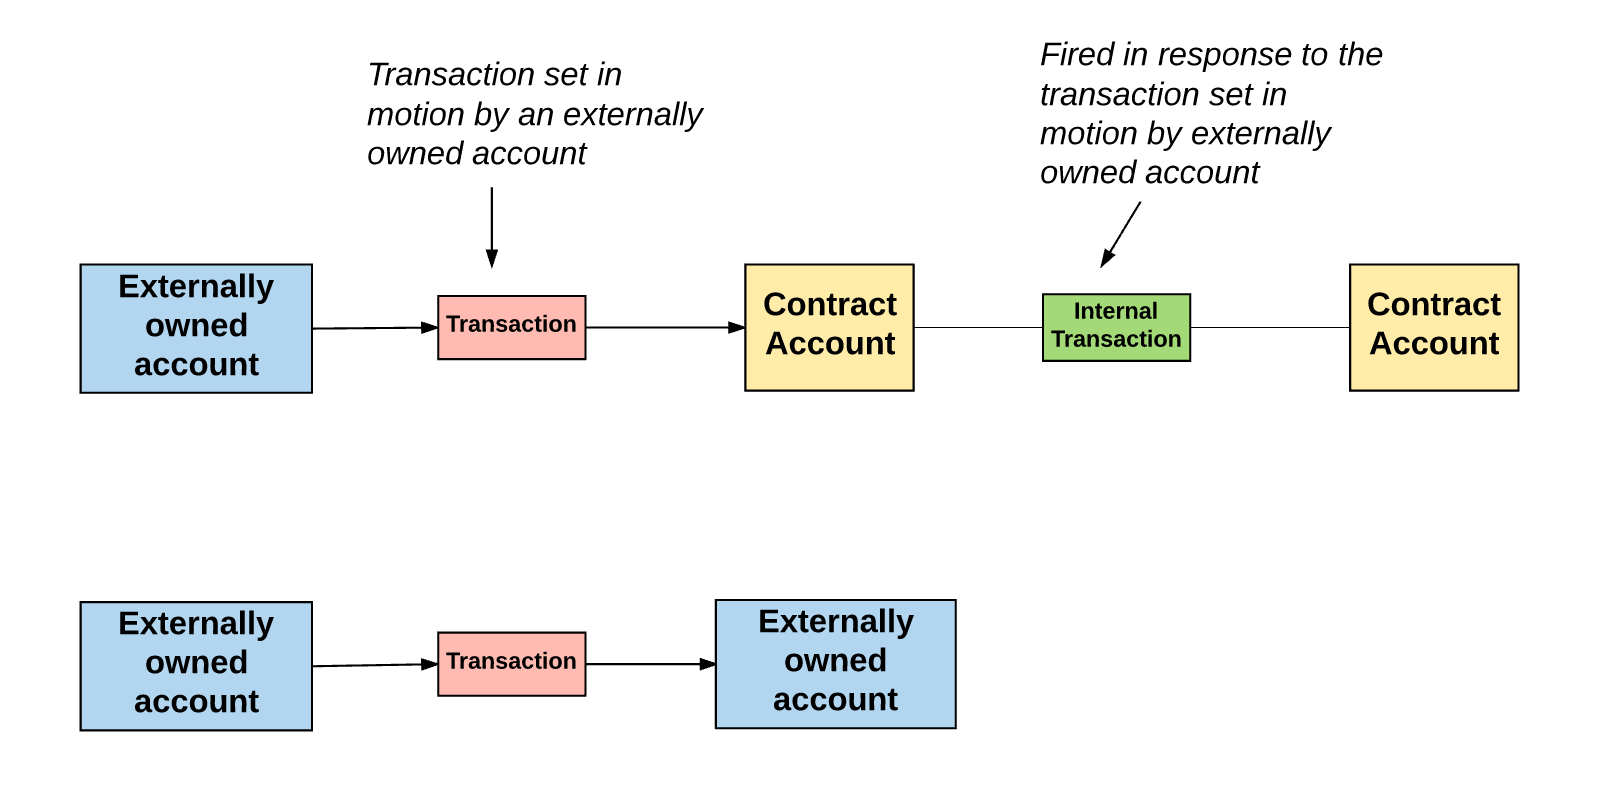
\includegraphics[width=1.0\textwidth]{result_tx}
    \caption{EOA can make a transaction to another EOA. A Contract fires a transaction after receiving a transaction from an EOA, from \cite{preethi}}
    \label{fig:tx_accounts}
\end{figure}

The public key of an EOA is derived from the private key through elliptic curve multiplication. The address of an EOA is calculated by calculating the KECCAK-256 hash of the public key and prefixing its last 20 bytes with `0x' \cite{ethereum}. The address of a CA is deterministically computed during contract creation from the sender EOA account's address and their transaction count\footnote{Full explanation: \url{https://ethereum.stackexchange.com/a/761}}.

We describe the contents of the Account State shown in Figure \ref{fig:accounts} as follows:
\begin{enumerate}
    \item \textbf{Nonce:} The number of transactions sent if it's an EOA, or the number of contracts created if it's a CA.
    \item \textbf{Balance:} The account's balance denominated in `wei'\footnote{1 ether $= 10^{18}$ wei }
    \item \textbf{Storage Hash:} The merkle root of the account's storage contents. This is empty for EOAs
    \item \textbf{Code Hash:} The hash of the code of the account. For EOAs this field is the KECCAK-256 hash of `' while for CAs it is the KECCAK-256 of the bytecode that exists at the CAs address.
\end{enumerate}

\subsection{Transactions} \label{transactions}
A transaction is a specially formatted data structure that gets signed by an EOA\footnote{With the EOAs private key} and gets broadcasted to an Ethereum node. Figure \ref{fig:transaction} shows the contents of a transaction as seen after querying an Ethereum node for its contents.

% In Bitcoin, the state is created through the Unspent Transaction Outputs set, which defines the amount of BTC  a user can spend. As Ethereum does not use UTXO but an account model, there needs to be a way to monitor the state. This is done through a data structure called Patricia State Trie \cite{Morrison:1968:PAR:321479.321481} which provides an efficient mapping of key and value pairs where the key is the address of the Ethereum account and the value is the Recursive Length Prefix encoding \cite{rlp} of the account's data. % TODO: Explain further or not? https://medium.com/cybermiles/diving-into-ethereums-world-state-c893102030ed %Whenever a transaction gets successfully mined, the world state gets updated accordingly.

Specifically:
\begin{enumerate}
    \item \textbf{blockHash:} The hash of the block that included the transaction.
    \item \textbf{blockNumber:} The number of the block that included the transaction.
    \item \textbf{from:} The transaction's sender\footnote{This field does not actually exist in a transaction however it is recovered from the v,r,s values of the signing algorithm (through \textit{ecrecover})}.
    \item \textbf{gas:} The maximum amount of gas that the sender will supply for the execution of the transaction (see \ref{gas}).
    \item \textbf{gasLimit:} The amount of Wei paid by the sender per unit of gas.
    \item \textbf{hash:} The transaction hash.
    \item \textbf{input:} Contains the data which is given as input to a smart contract in order to execute a function. Can also be used to embed a message in the transaction. Contains the value `0x0' in the case of simple transactions of ether.
    \item \textbf{nonce:} The number of transactions sent by the sender. It is used as a replay protection mechanism.
    \item \textbf{v, r, s:} Outputs of the ECDSA signature.
\end{enumerate}

\subsection{Blocks} \label{block}
A block contains the block header and a list of transaction hashes for all of the included transactions in that block. Figure \ref{fig:block} shows the contents of a transaction as seen after querying an Ethereum node for its contents.

Specifically:
\begin{enumerate}
    \item \textbf{difficulty:} The difficulty of the block.
    \item \textbf{extraData:} Extra data relevant to the block. Miners use it to claim credit for mining a block. In Bitcoin fields with extra data are used to let miners vote on a debate.
    \item \textbf{gasLimit:} The current maximum gas expenditure per block.
    \item \textbf{gasUsed:} The cumulative amount of gas used by all transactions included in the block.
    \item \textbf{hash:} The block's hash.
    \item \textbf{logsBlom:} A bloom filter which is used for getting further information from the transactions included in the block.
    \item \textbf{miner:} The address of the entity who mined the block.
    \item \textbf{mixHash:} A hash used for proving that the block has enough PoW on it.
    \item \textbf{nonce:} A number which when combined with the mixHash proves the validity of the block.
    \item \textbf{number:} The block's number.
    \item \textbf{parentHash:} The hash of the previous block's headers.
    \item \textbf{receiptsRoot:} The hash of the root node of the Merkle Tree containing the receipts of all transactions in the block .
    \item \textbf{sha3Uncles:} Hash of the uncles included in the block.
    \item \textbf{size:} Block size.
    \item \textbf{stateRoot:} The hash of the root node of the Merkle Tree containing the state (useful for light nodes).
    \item \textbf{totalDifficulty:} The cumulative difficulty of all mined blocks until the current block.
    \item \textbf{transactionsRoot:} The hash of the root node of the Merkle Tree containing all transactions in the block. 
\end{enumerate}

\subsection{Gas} \label{gas}
Since all nodes redundantly process all transactions and contract executions, an attacker would be able to maliciously flood the network with computationally intense transactions and cause nodes to perform costly operations for extended periods of time. Ethereum uses gas to introduce a cost on performing computations. Gas manifests itself as the fees to be paid by the sender for a transaction to complete successfully.

Every computational step on Ethereum costs gas. The simplest transaction which involves transferring Ether from one account to another costs 21000 gas. Calling functions of a contract involves additional operations where the costs can be estimated through the costs described in~\cite{gas, ethereum}. 

When referring to blocks, the \textit{gasLimit} is the maximum gas that can be included in a block. Since each transaction consumes a certain amount of gas, the cumulative gas used by all transactions in a block needs to be less than \textit{gasLimit}. There is a similarity between the block gasLimit and the block size in Bitcoin in that they are both used to limit the amount of transactions that can be included in a block. The difference in Ethereum is that miners can `vote' on the block gasLimit.

Every unit of gas costs a certain amount of \textit{gasPrice} which is set by the sender of the transaction. The cost of a transaction in wei is calculated from the following formula:
\begin{equation}
    totalTransactionCost = gasPrice * gasUsed
\end{equation}
\begin{quote}
    \noindent
    where $gasUsed$ is the amount of gas consumed by the transaction
\end{quote}

Miners are considered to be rational players who are looking to maximize their profit. As a result, they are expected to include transactions with transaction costs before transactions with low transaction costs. This effectively creates a `fee market'  where users are willing to pay more by increasing the \textit{gasPrice} to have their transactions confirmed faster. In the times of network congestion such as popular Initial Coin Offerings\footnote{Crowdfunding for cryptocurrency projects which allow investors to buy tokens in a platform}\cite{batico} or mass-driven games such as CryptoKitties\footnote{\url{https://cryptokitties.co}}\cite{cryptokitties} transactions become very expensive and can take long times to confirm.

\subsubsection{Successful Transaction}
In the case of a successful transaction, the consumed gas from \textit{gasLimit} (\textit{gasUsed}) goes to miners, while the rest of the gas gets refunded to the sender. After the completion, the world state gets updated.

\begin{figure}[H]
    \centering
    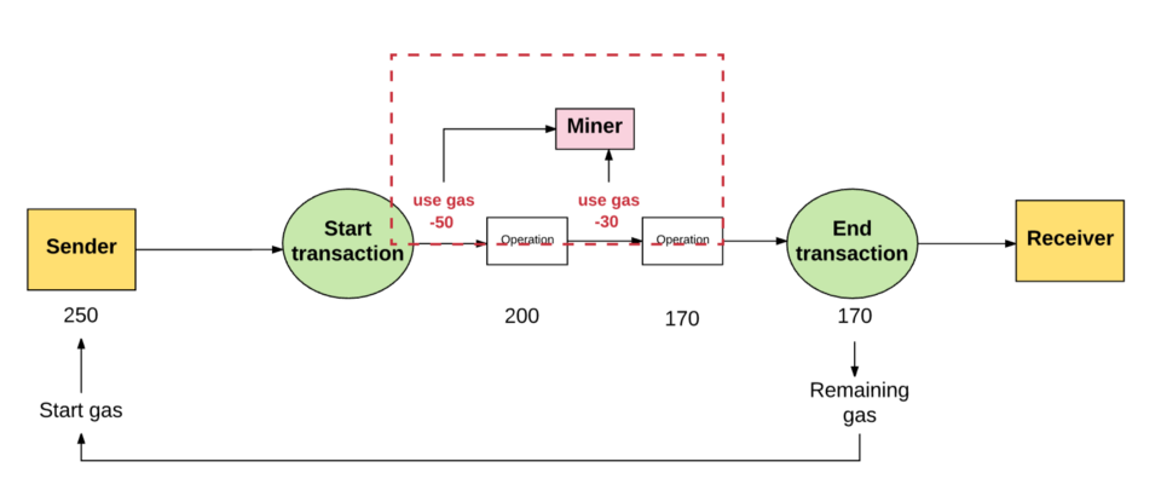
\includegraphics[width=1.0\textwidth]{successful_tx}
    \caption{Successful transaction, from \cite{preethi}}
    \label{fig:successful_tx}
\end{figure}

\subsubsection{Failed Transaction}
A transaction can fail for reasons such as not being given enough gas for its computations, or some exception occurring during its execution. In this case, any gas consumed goes to the miners and any state changes that would happen are reverted. This is similar to the SQL transaction commit-rollback pattern.

\begin{figure}[H]
    \centering
    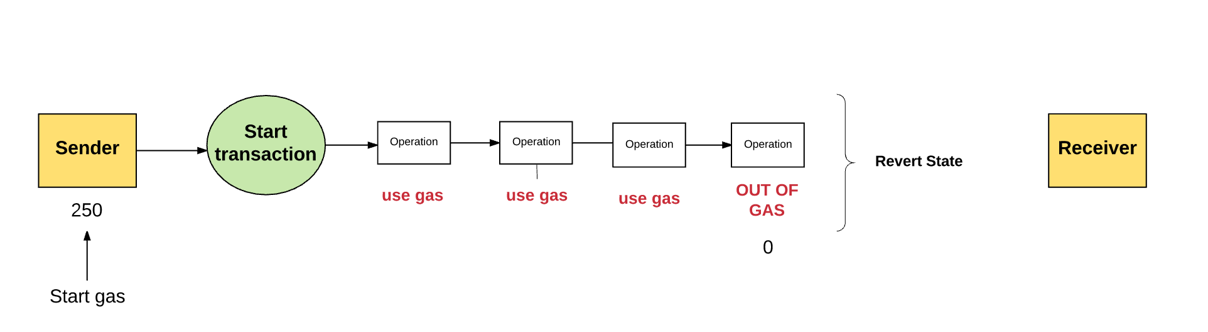
\includegraphics[width=1.0\textwidth]{nogas_tx}
    \caption{Failed transaction that ran out of gas, from \cite{preethi}}
    \label{fig:nogas_tx}
\end{figure}

\subsection{Mining}
The set of rules which allow an actor to add a valid block to the blockchain is called a \textit{consensus algorithm}. In order to have consensus in distributed systems, all participating nodes must have the same version (often called history) of the system (blockchain). If there were no rules for block creation, a malicious node would be able to consistently censor transactions or double-spend \cite{doublespend}. In order to avoid that, consensus algorithms elect a network participant to decide on the contents of the next block. 

Ethereum uses a consensus algorithm called ethash\cite{ethash} which is a memory-hard\footnote{Requires a large amount of memory to execute it. This means that creating ASICs for ethash is harder, although not impossible \cite{asicfork}} consensus algorithm which requires a valid PoW in order to append a block to the Ethereum blockchain. PoW involves finding an input called \textit{nonce} to the algorithm so that the output number is less than a certain threshold\footnote{The threshold is also called difficulty and adjusts dynamically so that a valid PoW is found approximately every 12.5 seconds}. PoW algorithms are designed so that the best strategy to find a valid nonce is by enumerating through all the possible options. Finding a valid PoW is a problem that requires a lot of computational power, however verifying a solution is a trivial process, given the nonce. In return, miners are rewarded with the \textit{block reward} and with all the fees from the block's transactions.

This process is called `mining'. In the future, Ethereum is planning to transition to another \textit{consensus algorithm} called Proof of Stake (PoS), which deprecates the concept of `mining' and replaces it with `staking'. PoS is considered to be a catalyst for achieving scalability in blockchains and is briefly discussed in Chapter \ref{ch:scalability}.

%%%%%%%%%%%%%%%%%%%%%%%%%%%%%%%%%%%%%%%%%

\section{Programming in Ethereum}
At a low level, the EVM has its own Turing Complete language called the EVM bytecode. Programmers write in higher-level languages and compile the code from them to EVM bytecode which gets executed by the EVM\@.

\subsection{Programming Languages}
Languages that compile to EVM code are Solidity, Serpent, LLL or Vyper. 

Solidity is the most popular language in the ecosystem and although often comparable to Javascript, we argue that Solidity Smart Contracts remind more of C++ or Java, due to their object oriented design. The Solidity Compiler is called \textit{solc}. In order to deploy a smart contract, its EVM Bytecode and its Application Binary Interface (ABI) are needed, which can be obtained from the compiler.

\begin{figure}[ht]
    \centering
    \lstinputlisting[language=Solidity]{contracts/example1.sol}
    \caption{Basic Solidity Smart Contract}
    \label{fig:smart_contract}
\end{figure}

Due to the nascence of these languages and the security mistakes that have occurred due to them providing programmers with powerful state-changing functions, active research is being done towards safer languages~\cite{bamboo}.

\subsection{Tooling}
The following section describes tools and software that are often used by Ethereum users and developers to interact with the network.

\subsubsection{Client (Node) Implementations and Testnets}
Ethereum's official implementations are Geth (golang) and cpp-ethereum (C++). Third party implementations such as Parity (Rust), Pyethereum (Python) and EthereumJ (Java) also exist. The most used kind of node implementations are Geth (compatible with Rinkeby testnet) and Parity (compatible with Kovan testnet). 

Smart contracts are immutable once deployed which means that their deployed bytecode (and thus their functionality) cannot change. As a result, if a flaw is found on a deployed contract, the only way to fix it is by deploying a new contract. In addition, the deployment costs can be expensive, so development and iterative testing can be costly. For that, public test networks (testnets) exist which allow for testing free of charge. Kovan and Rinkeby are functioning with the Proof of Authority \cite{poa} consensus algorithm, while Ropsten is running Ethash \cite{ethash} with less difficulty.

We provide a comparison between test networks:
\begin{enumerate}
    \item Kovan: Proof of Authority consensus supported by Parity nodes only
    \item Rinkeby: Proof of Authority consensus supported by Geth nodes only
    \item Ropsten: Proof of Work consensus, supported by all node implementations, provides best simulation to the main network 
    % https://ethereum.stackexchange.com/questions/27048/comparison-of-the-different-testnets
\end{enumerate}
% https://ethereum.stackexchange.com/questions/27048/comparison-of-the-different-testnets

In addition, before deploying to a testnet, developers are encouraged to run their own local testnets. Geth and Parity allow for setting up private testnets. Third-party tools also exist that allow for setting up a blockchain with instant confirmation times and prefunded accounts, such as ganache\footnote{\url{http://truffleframework.com/ganache}}(User Interface at \ref{fig:ganache},  formerly known as testrpc).


\subsubsection{Web3}
Web3 is the library used for interacting with an Ethereum node. The most feature-rich implementation is Web3.js\footnote{\url{https://github.com/ethereum/web3.js}} which is also used for building web interfaces for Ethereum Decentralized Applications (DApps). Implementations for other programming languages are being worked on such as Web3.py\footnote{\url{https://github.com/ethereum/web3.py}}. We illustrate an example of connecting and fetching the latest block from Ropsten and Mainnet using Web3.js in \ref{fig:web3js} and Web3.py in \ref{fig:web3py}. The full specifications of each library's API can be found in their respective documentation\footnote{\url{https://github.com/ethereum/wiki/wiki/JavaScript-API}}\footnote{\url{https://web3py.readthedocs.io/en/stable/}}


\subsubsection{Truffle Framework}
The Truffle Framework is a development framework for smart contract development written in NodeJS. It is currently the industry standard for developers. It allows for automating the smart contract deployment pipeline through \textit{migration} scripts and scripting test suites for scenarios using the Mocha Testing suite. Finally, it includes a debugger for stepping through transaction execution and can internally launch a ganache testnet.

\section{Related Work}
Techniques which illustrate more efficient smart contracts by storing less data on a blockchain are described in~\cite{stateless}. \cite{DBLP:journals/corr/ChenLLZ17} makes it clear that compiler optimizations in smart contracts still need improvements in order to avoid unnecessary expenses. On network level scalability there are various approaches such as executing transactions `off-chain'\footnote{An exchange of cryptographically signed messages that does not happen on a blockchain.}~\cite{raiden, funfair, counterfactual} and use a blockchain only for the final settling of a series of transactions. Other approaches exist which involve creating `sidechains' which can be used to offload the computational effort from the `mainchain' \cite{sidechains, loom, cosmos, plasmacash, plasma}. Finally, another approach to achieving scalability is via permissioned blockchains which trade decentralization and transparency for efficiency~\cite{hyperledger, Vukolic:2017:RPB:3055518.3055526}.

Extensive analyses have been performed on the security of blockchains as networks~\cite{Gervais:2016:SPP:2976749.2978341, cryptoeprint:2018:236} and specifically on the security of Ethereum smart contracts~\cite{Atzei:2017:SAE:3080353.3080363} which have proven to be insufficiently secure for the amounts of funds that they hold. As a result, tools that are able to analyze both source code and compiled bytecode for vulnerabilities have been developed~\cite{Luu:2016:MSC:2976749.2978309, mythril, echidna, smartcheck, securify, zeus}. A recent study \cite{greedyprodigal} illustrates how smart contracts that can freeze or cause loss of funds can be detected \cite{maian}.

Utilizing blockchain for Internet of Things is explored in \cite{iot, integrationiot}, while a model for billing and accounting with smart contracts is proposed in~\cite{billaccount}. Energy market use-cases are being piloted by~\cite{gridplus, powerledger} and prototypes are being tested such as \cite{brooklyn, DBLP:journals/ife/MengelkampNBDW18}.